\documentclass[tikz,border=9pt,12pt]{standalone}
\usepackage{amsmath,amssymb}
\usetikzlibrary{arrows.meta,calc}
\tikzset{every node/.style={text=black,font=\normalsize},axis/.style={-{Stealth[length=2mm]},black!65,thin},vec/.style={-{Stealth[length=2.8mm]},line width=1.3pt,blue!70!black},lab/.style={fill=white,inner sep=2pt}}
\begin{document}
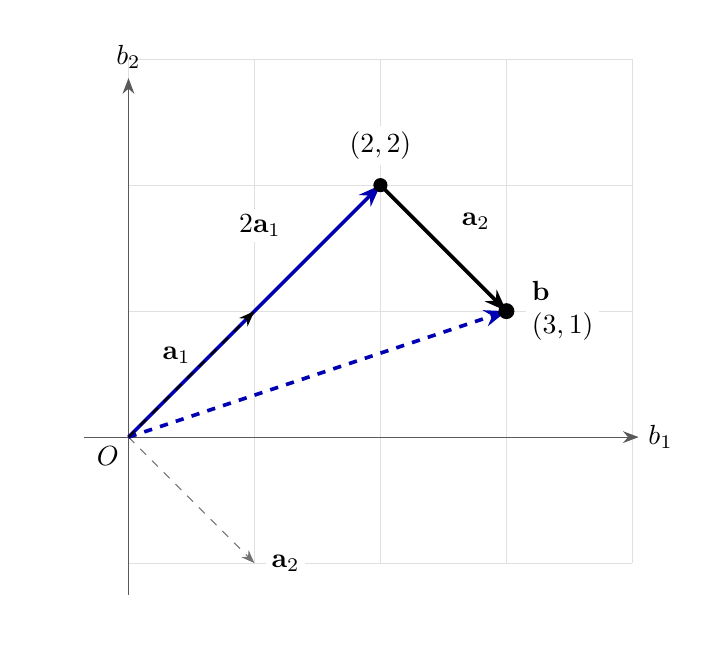
\begin{tikzpicture}[scale=1.6]
\path[use as bounding box] (-.8,-1.55) rectangle (4.45,3.25);
\draw[step=1,black!12,very thin] (0,-1) grid (4,3);
\draw[axis] (-.35,0)--(4.05,0) node[right] {$b_1$};
\draw[axis] (0,-1.25)--(0,2.85) node[above] {$b_2$};
\node[below left] at (0,0) {$O$};

\node[lab,left=5pt] at (.65,.65) {$\mathbf a_1$};
\draw[black!55,dashed,-{Stealth}] (0,0)--(1,-1);
\node[lab,right=4pt] at (1,-1) {$\mathbf a_2$};
\draw[vec] (0,0)--(2,2) node[pos=.70,above left=6pt,lab] {$2\mathbf a_1$};
\draw[-{Stealth[length=2.8mm]},black,line width=1.3pt] (2,2)--(3,1) node[midway,above right=4pt,lab] {$\mathbf a_2$};
\draw[vec,dashed] (0,0)--(3,1);
\draw[black,dashed,-{Stealth[length=2mm]},line width=.8pt] (0,0)--(1,1);
\fill (2,2) circle (1.6pt);
\node[lab,above=7pt] at (2,2) {$(2,2)$};
\fill (3,1) circle (1.8pt);
\node[lab,right=7pt,align=left] at (3,1) {$\mathbf b$\\$(3,1)$};
\end{tikzpicture}
\end{document}
